\section{HIGH-\pt\ PARTICLE SPECTRA}
\label{spectra}
Transverse momentum spectra of charged particles were measured by all three experiments with the first collected data sample. They are presented as the dependence of the inclusive invariant cross section or yield on the transverse momentum ($p_{\rm T}$), and finally in a form normalized to pp measurement at the same nucleon--nucleon energy: the nuclear modification factor, defined as
\be
R_{\rm AA}(p_{\rm T}) = \frac{{\rm d}N_{\rm ch}^{\rm AA}(p_{\rm T})/{\rm d}p_{\rm T}}{\langle N_{\rm coll} \rangle \,{\rm d}N_{\rm ch}^{\rm pp}(p_{\rm T})/{\rm d}p_{\rm T}}\, ,
\label{eqks:RAA}
\ee
where on the right hand side the superscripts AA and pp at the charged particle yield $N_{\rm ch}$ refer to the values obtained in heavy-ion and pp measurements, respectively, while $\langle N_{\rm coll} \rangle$ denotes the average number of binary collisions for a selection for which the \Raa\ is evaluated. The number of binary collisions $N_{\rm coll}$ is calculated together with the number of participants $N_{\rm part}$ using the Glauber Monte Carlo method~\cite{Shor:1988vk,Alver:2008aq}, which is exploited for the determination of collision centrality~\cite{Miller:2007ri,Abelev:2013qoq}. Centrality selection is usually expressed as a percentage (or a range of percentages) of total nuclear cross section corresponding to the fraction of the most central collisions (or a range between two such fractions, when the selection does not represent the top central collisions). A natural expectation for hard processes, in case that nucleons act independently and their interactions are not influenced by the rest of the nuclei, is that the yields scale with $N_{\rm coll}$, and thus the nuclear modification factor would be $R_{\rm AA} = 1$. This is observed for non-strongly interacting particles (electro-weak bosons, direct photons), since they are practically not influenced by the surrounding medium, see Sec.~\ref{sect:pas:ew}.
\subsection{Charged-Particle Spectra}
\label{subsecks:transspectra}
The $p_{\rm T}$ spectrum for charged particles in LHC heavy-ion collisions was expected to be suppressed at high $p_{\rm T}$ with respect to pp interactions. The fact that $R_{\rm AA}$ is significantly below unity at $p_{\rm T}$ above a few GeV had been well established for central collisions at RHIC, and attributed to jet quenching --- an energy loss of hard partons in their interactions with the surrounding high-density nuclear matter. Since high-$p_{\rm T}$ particles are supposed to be produced in the fragmentation of such hard partons, having steeply falling \pt\ spectrum, their quenching lowers the particle production, reflecting the amount of energy loss, and thus the density of nuclear matter created in the collision. However, the value of $R_{\rm AA}$ is also dependent on the steepness of the parton $p_{\rm T}$ spectrum (a harder parton spectrum at the LHC should result in less particle suppression), and on the nuclear modification of the structure functions (distribution of partons inside a nucleon). Therefore, for theoretical predictions and interpretations of the $R_{\rm AA}$ behavior, model calculations taking into account the interplay of many effects are necessary.

The first LHC measurement of charged-particle $R_{\rm AA}$, was published by ALICE~\cite{Aamodt:2010jd}, presenting the $p_{\rm T}$ spectrum up to 20~GeV, for the 5\,\% most central Pb--Pb events. It showed a slightly stronger suppression compared to RHIC: the largest suppression, in the $p_{\rm T}$ range 6--7~GeV, was a factor about 7 at the LHC, while at RHIC a factor of 5 was observed. A new observation was that with increasing $p_{\rm T}$ the suppression becomes smaller, i.e. $R_{\rm AA}$ increases. This was soon confirmed by the CMS measurement~\cite{CMS:2012aa}, extending the $p_{\rm T}$ reach up to 100~GeV (see Fig.~\ref{figks:CMSRAA}). The nuclear modification factor $R_{\rm AA}$ exhibits a clear increase up to $p_{\rm T}$ about 40~GeV, and then seems to saturate at a value about 0.5--0.6 for the most central collisions. Figure~\ref{figks:CMSRAA} also shows the $p_{\rm T}$ dependence of $R_{\rm AA}$ at lower energies, and a variety of model calculations~\cite{Dainese:2004te,Vitev:2002pf,Vitev:2004bh,Salgado:2003gb,Armesto:2005iq,Renk:2011gj}. Different models can be tuned to fairly reproduce the $R_{\rm AA}$ data, however, it remains to be demonstrated that they describe with the same parameters the ensemble of other observables, especially the azimuthal anisotropy.

\begin{figure}[!ht]
\centering
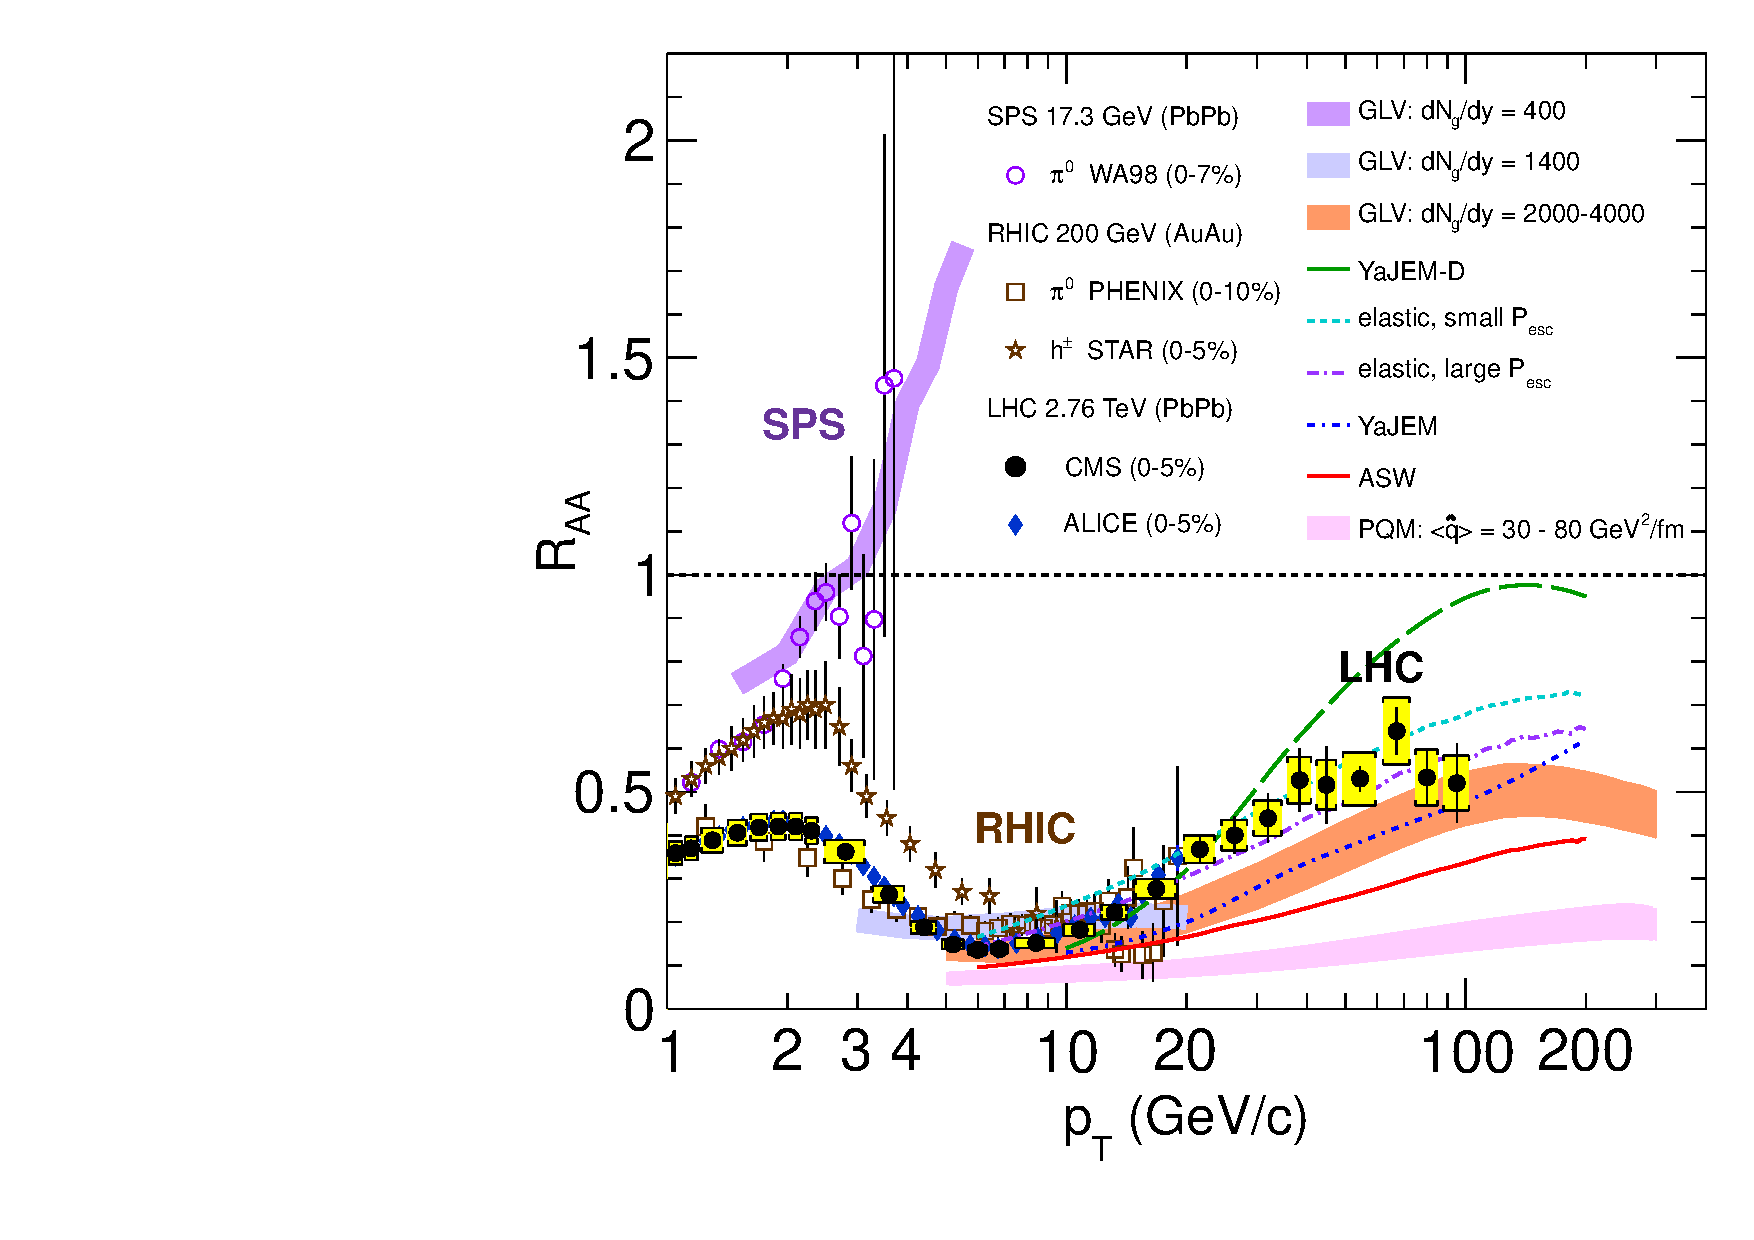
\includegraphics[width=0.5\textwidth]{particlefigs/CMSRAA.pdf}
\caption{Transverse momentum dependence of nuclear modification factor $R_{\rm AA}$ for charged particles produced in central heavy-ion collisions at LHC and lower energies. The curves and bands represent different model calculations. Reproduced from~\cite{CMS:2012aa}.}
\label{figks:CMSRAA}
\end{figure}

The CMS and ALICE experiments also measured the $R_{\rm AA}$ $p_{\rm T}$ dependence for different collision centralities~\cite{CMS:2012aa,Abelev:2012hxa}. The charged-particle production is, as expected, less and less suppressed as one moves from central to peripheral Pb--Pb collisons. The ATLAS collaboration has reported similar results, presented as $R_{\rm CP}$ as a function of $p_{\rm T}$, where $R_{\rm CP}$ stands for a quantity analogue  to that defined in Eq.~\ref{eqks:RAA} using the normalized ratio of heavy-ion results at different centralities (the subscript CP indicates the central-to-peripheral ratio), commonly using the most peripheral available class for normalization.
%R_AA from CMS up to 100 GeV
\subsection{Identified-Hadron Spectra}
\label{subsecks:identspectra}
The study of the particle composition as a function of $p_{\rm T}$ reveals a mass hierarchy, interpreted as resulting from a common radial-velocity flow created during the expansion of the dense-matter fireball. Such collective flow arises in strongly interacting matter in the presence of a pressure gradient. For a given velocity profile, heavier particles (e.g. protons) will acquire a larger momentum than lighter mesons. The effect should be largest at low \pt\ and should disappear progressively with increasing \pt\ (for $p_{\rm T}$ values significantly larger than particle masses).

\begin{figure}[!ht]
\centering
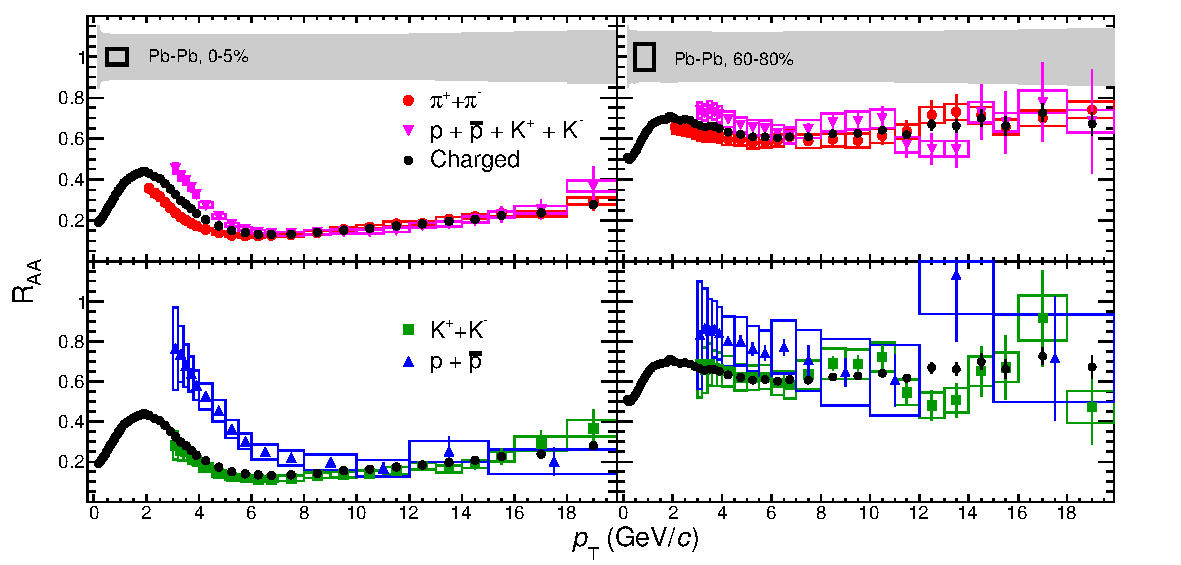
\includegraphics[width=0.7\textwidth]{particlefigs/IdentHighPtRAA.pdf}
\caption{Nuclear modification factor $R_{\rm AA}$ for pions, kaons, and protons (sum of particles and antiparticles), and averaged for charged particles, as a function of $p_{\rm T}$ for central (left, 0--5\,\%) and peripheral (right, 60--80\,\%) Pb--Pb collisions. Reproduced from~\cite{ALICEIdentHighPtRAA}.}
\label{figks:IdentPartRAA}
\end{figure}

The $p_{\rm T}$ spectra of identified charged hadrons are determined up to $p_{\rm T} = 20$~GeV~\cite{ALICEIdentHighPtRAA}. Figure~\ref{figks:IdentPartRAA} presents these results as $R_{\rm AA}$ for pions, kaons, and protons, compared to the (averaged) charged-particle data. It is clearly seen that for $p_{\rm T}$ above 7--8~GeV the behaviors for all particle species coincide. For lower $p_{\rm T}$ a mass hierarchy appears: the heavier the particle, the lower its suppression. A similar conclusion holds also for production of strange particles, such as $\Lambda$, $\Xi$, and $\Omega$~\cite{ABELEV:2013zaa,Abelev:2013xaa}. These observations suggest the existence of three regions in transverse momentum:
\begin{itemize}
    \item{bulk region, low $p_{\rm T}$ up to 2--3~GeV, where the production is dominated by the hadronization of high-density strongly-interacting matter created in a heavy-ion collision, reflecting collective radial flow, fairly well described (at least for central collisions) by hydrodynamical models;}
    \item{intermediate region, in $p_{\rm T}$ up to 7--8~GeV, where a mass splitting among various particle species still persists, that could be attributed a reminiscence of radial flow; however, additional ideas were put forward, such as constituent-quark recombination, to increase the $p_{\rm T}$ range of this mass distinction;}
    \item{fragmentation region, above 7--8~GeV in $p_{\rm T}$, where the different hadron species exhibit a common suppression pattern, and consequently their relative abundances are the same as in pp collisions, naturally explained as being fragmentation products of a high-$p_{\rm T}$ parton coming from a hard scattering at early stage (itself quenched by the surrounding high-density matter).}
\end{itemize}

A detailed investigation of the intermediate region has been performed by the measurement of the \pt\ dependence of the proton-to-pion~\cite{ALICEIdentHighPtRAA} and $\Lambda$-to-kaon~\cite{Abelev:2013xaa} ratios. For central collisions at $p_{\rm T}$ around 2.5--3~GeV these ratios are more than a factor three higher than the corresponding values for pp collisions. This so-called baryon anomaly was observed already at RHIC~\cite{Abelev:2006jr,Adare:2013esx}, and the low-$p_{\rm T}$ rise is well understood based on the hydrodynamical radial flow. In the intermediate region, where hydrodynamics ceases to work, the behavior is qualitatively described by models involving constituent-quark recombination~\cite{Fries:2003kq,Hwa:2006zq,Song:2007ux} or baryon string-junction transfer along the axis of a fragmenting jet~\cite{Aurenche:2011rd}. Recently, a good description has been obtained by EPOS model~\cite{Werner:2012xh}, where the interaction between bulk matter and jets is considered.
\subsection{High-\pt\ Particle Correlations}
\label{subsecks:correlation}
Two-particle correlations are used to study parton quenching at $p_{\rm T}$ below ${\cal O}(10)$~GeV~\cite{Aamodt:2011vg}, where full jet reconstruction is difficult due to the underlying event fluctuations~\cite{Abelev:2012ej}. The correlation in the relative azimuthal angle $\Delta\varphi$ between a trigger particle within $8 < p_{\rm T}^{\rm t} < 15$~GeV and the associated particles with transverse momentum $p_{\rm T}^{\rm a}$, respecting $p_{\rm T}^{\rm a} <p_{\rm T}^{\rm t}$, has been studied~\cite{Aamodt:2011vg}. In order to measure the number of associated particles correlated with the trigger particle on the near-side and the away-side jet structures, the distribution after background subtraction is integrated around the near- and away-side peaks, in the $\Delta\varphi$ intervals $\pm 0.7$ and $\pi \pm 0.7$, respectively. The per-trigger yields of associated particles, obtained this way, normalized to the corresponding yields measured in pp collisions, represent the nuclear modification factor of the conditional yields, $I_{\rm AA}$. 
%The near- and away-side $I_{\rm AA}$ are presented in Fig.~\ref{figks:IAA} as a function of associated-particle %$p_{\rm T}^{\rm a}$. 
The results are practically independent on $p_{\rm T}^{\rm a}$, and for peripheral collisions compatible with no nuclear modification. For central collisions, the away-side $I_{\rm AA}$ is around 0.6, which is interpreted as a manifestation of jet quenching. On the near-side an enhancement for Pb--Pb with respect to pp collisions is observed, which could be understood a consequence of a modification of the fragmentation function, possibly caused by jet quenching and a trigger bias. This measurement constrains various parton-quenching models, some recently reported a fair description of such effect~\cite{Renk:2011wp}.

%\begin{figure}[!ht]
%\centering
%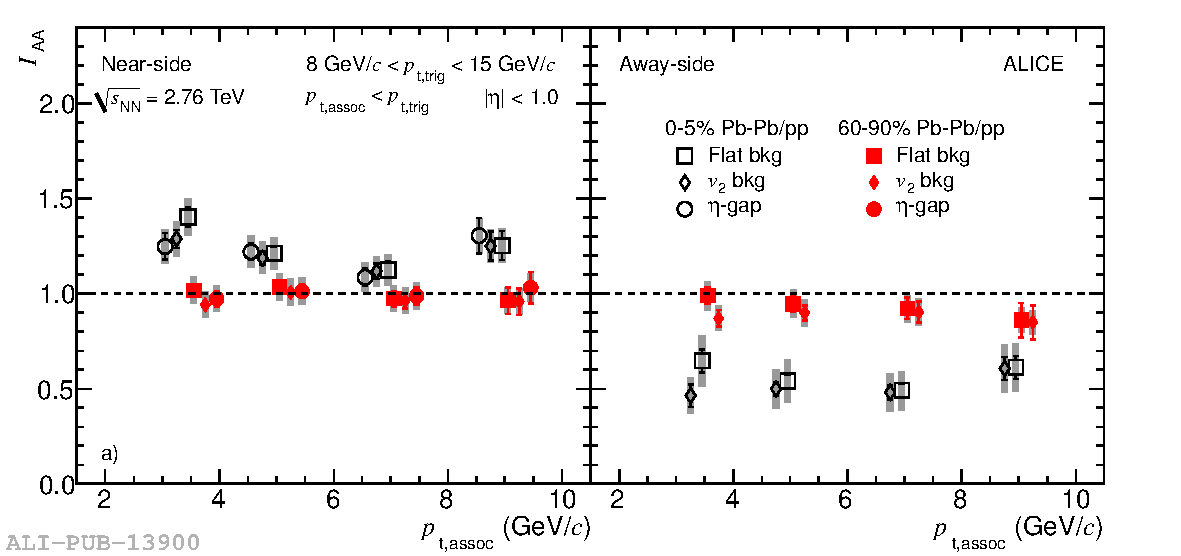
\includegraphics[width=0.7\textwidth]{particlefigs/IAA.pdf}
%\caption{Near-side (left) and away-side (right) $I_{\rm AA}$ as a function of the transverse momentum of associated %particles. The results are shown for peripheral (60--90\,\%) and central (0--5\,\%) Pb--Pb collisions. The three %values shown for each measurement correspond to three background subtraction methods. Reproduced %from~\cite{Aamodt:2011vg}.}
%\label{figks:IAA}
%\end{figure}

The triggered two-particle correlations in two dimensions, $\Delta\varphi$ and $\Delta\eta$ (pseudorapidity difference between trigger and associated particles), have been exploited to study the shape of the jet-structures~\cite{Morsch:2012gb}. The $\Delta\eta$ jet-structure width increases with the centrality of Pb--Pb collisions, while in the $\Delta\varphi$ direction no strong increase is observed. This could be explained by a jet interaction with longitudinally flowing medium~\cite{Armesto:2004pt}. The particle composition of such jet-like structures is important for the understanding of the in-medium modification of parton fragmentation. The proton-to-pion ratio has been measured in $(\Delta\varphi, \Delta\eta)$ regions, both inside and outside the jet structures selected in the correlation plot~\cite{Veldhoen:2012ge}. The jet p/$\pi$ ratio is obtained by correcting the jet-region value with properly weighted outside-jet (bulk) measurements. While the bulk p/$\pi$ ratio reproduces the baryon anomaly (see Sec.~\ref{subsecks:identspectra}), the jet ratio is compatible with the expectation for the jet fragmentation in pp collisions.
